\chapter{Worked example: infer SAF microarchitecture topology from architecture and SAFs}
\label{appendix:safinfer_build}

This section provides a worked example of SAFinfer taxonomic inference.

The steps are as follows:
\begin{itemize}
    \item Sparseloop-style declarative specification of architecture and SAF optimizations. Figure~\ref{fig:safinfer_build_00saf}
    \item Concretization rule: replace declarative specs with high-level SAF microarchitecture blocks (FMT,SKIP.) Figure~\ref{fig:safinference_build_01concretization}
    \item Port format(s) from attribute(s) rule: infer FMT block port formats from \textit{fmt\_list} attribute. Figure~\ref{fig:safinference_build_02fmtporttype}
    \item Topology inference from customization rule: infer FMT block implementation topology based on customization. Figure~\ref{fig:safinference_build_03fmttopology}
    \item Wire-transitive rule: infer mdparsers' port formats from FMT block ports' formats. Figure~\ref{fig:safinference_build_04mdparserportfmt}
    \item Attribute from port format rule: infer mdparsers \textit{format} attributes' values from mdparsers ports' formats. Figure~\ref{fig:safinference_build_05mdparserfmtattr}
    \item User customization rule: mdparsers' \textit{strategy} attributes are user-configurable free parameters. Figure~\ref{fig:safinference_build_06mdparserstratcust}
    \item Wire-transitive rule: infer architectural buffer-stub ports' formats from FMT block ports' formats. Figure~\ref{fig:safinference_build_07buffportfmt}
    \item Wire-transitive rule: infer SKIP block ports' formats from architectural buffer stub ports' formats. Figure~\ref{fig:safinference_build_08skipportfmt}
    \item Attribute from port format rule: infer SKIP block format attributes' values from SKIP blocks ports' formats. Figure~\ref{fig:safinference_build_09skipfmtattrs}
    \item User customization rule: SKIP block's \textit{optimize\_fills} attribute is a user-configurable free parameter. Figure~\ref{fig:safinference_build_10skipoptfillscust}
    \item Topology inference from customization rule: infer SKIP block implementation topology based on customization. Figure~\ref{fig:safinference_build_11skiptopology}
    \item Process-of-elimination rule: isectlf and both pgen1 units have only one supported customization; fill in unknown attributes. Figure~\ref{fig:safinference_build_12isectlfpgenoneopt}
    \item User customization rule: fopt's \textit{strategy} attribute is a user-configurable free parameter. SAF microarchitecture taxonomic inference is complete. Figure~\ref{fig:safinference_build_13foptstratcust}
\end{itemize}

\begin{figure}[H]
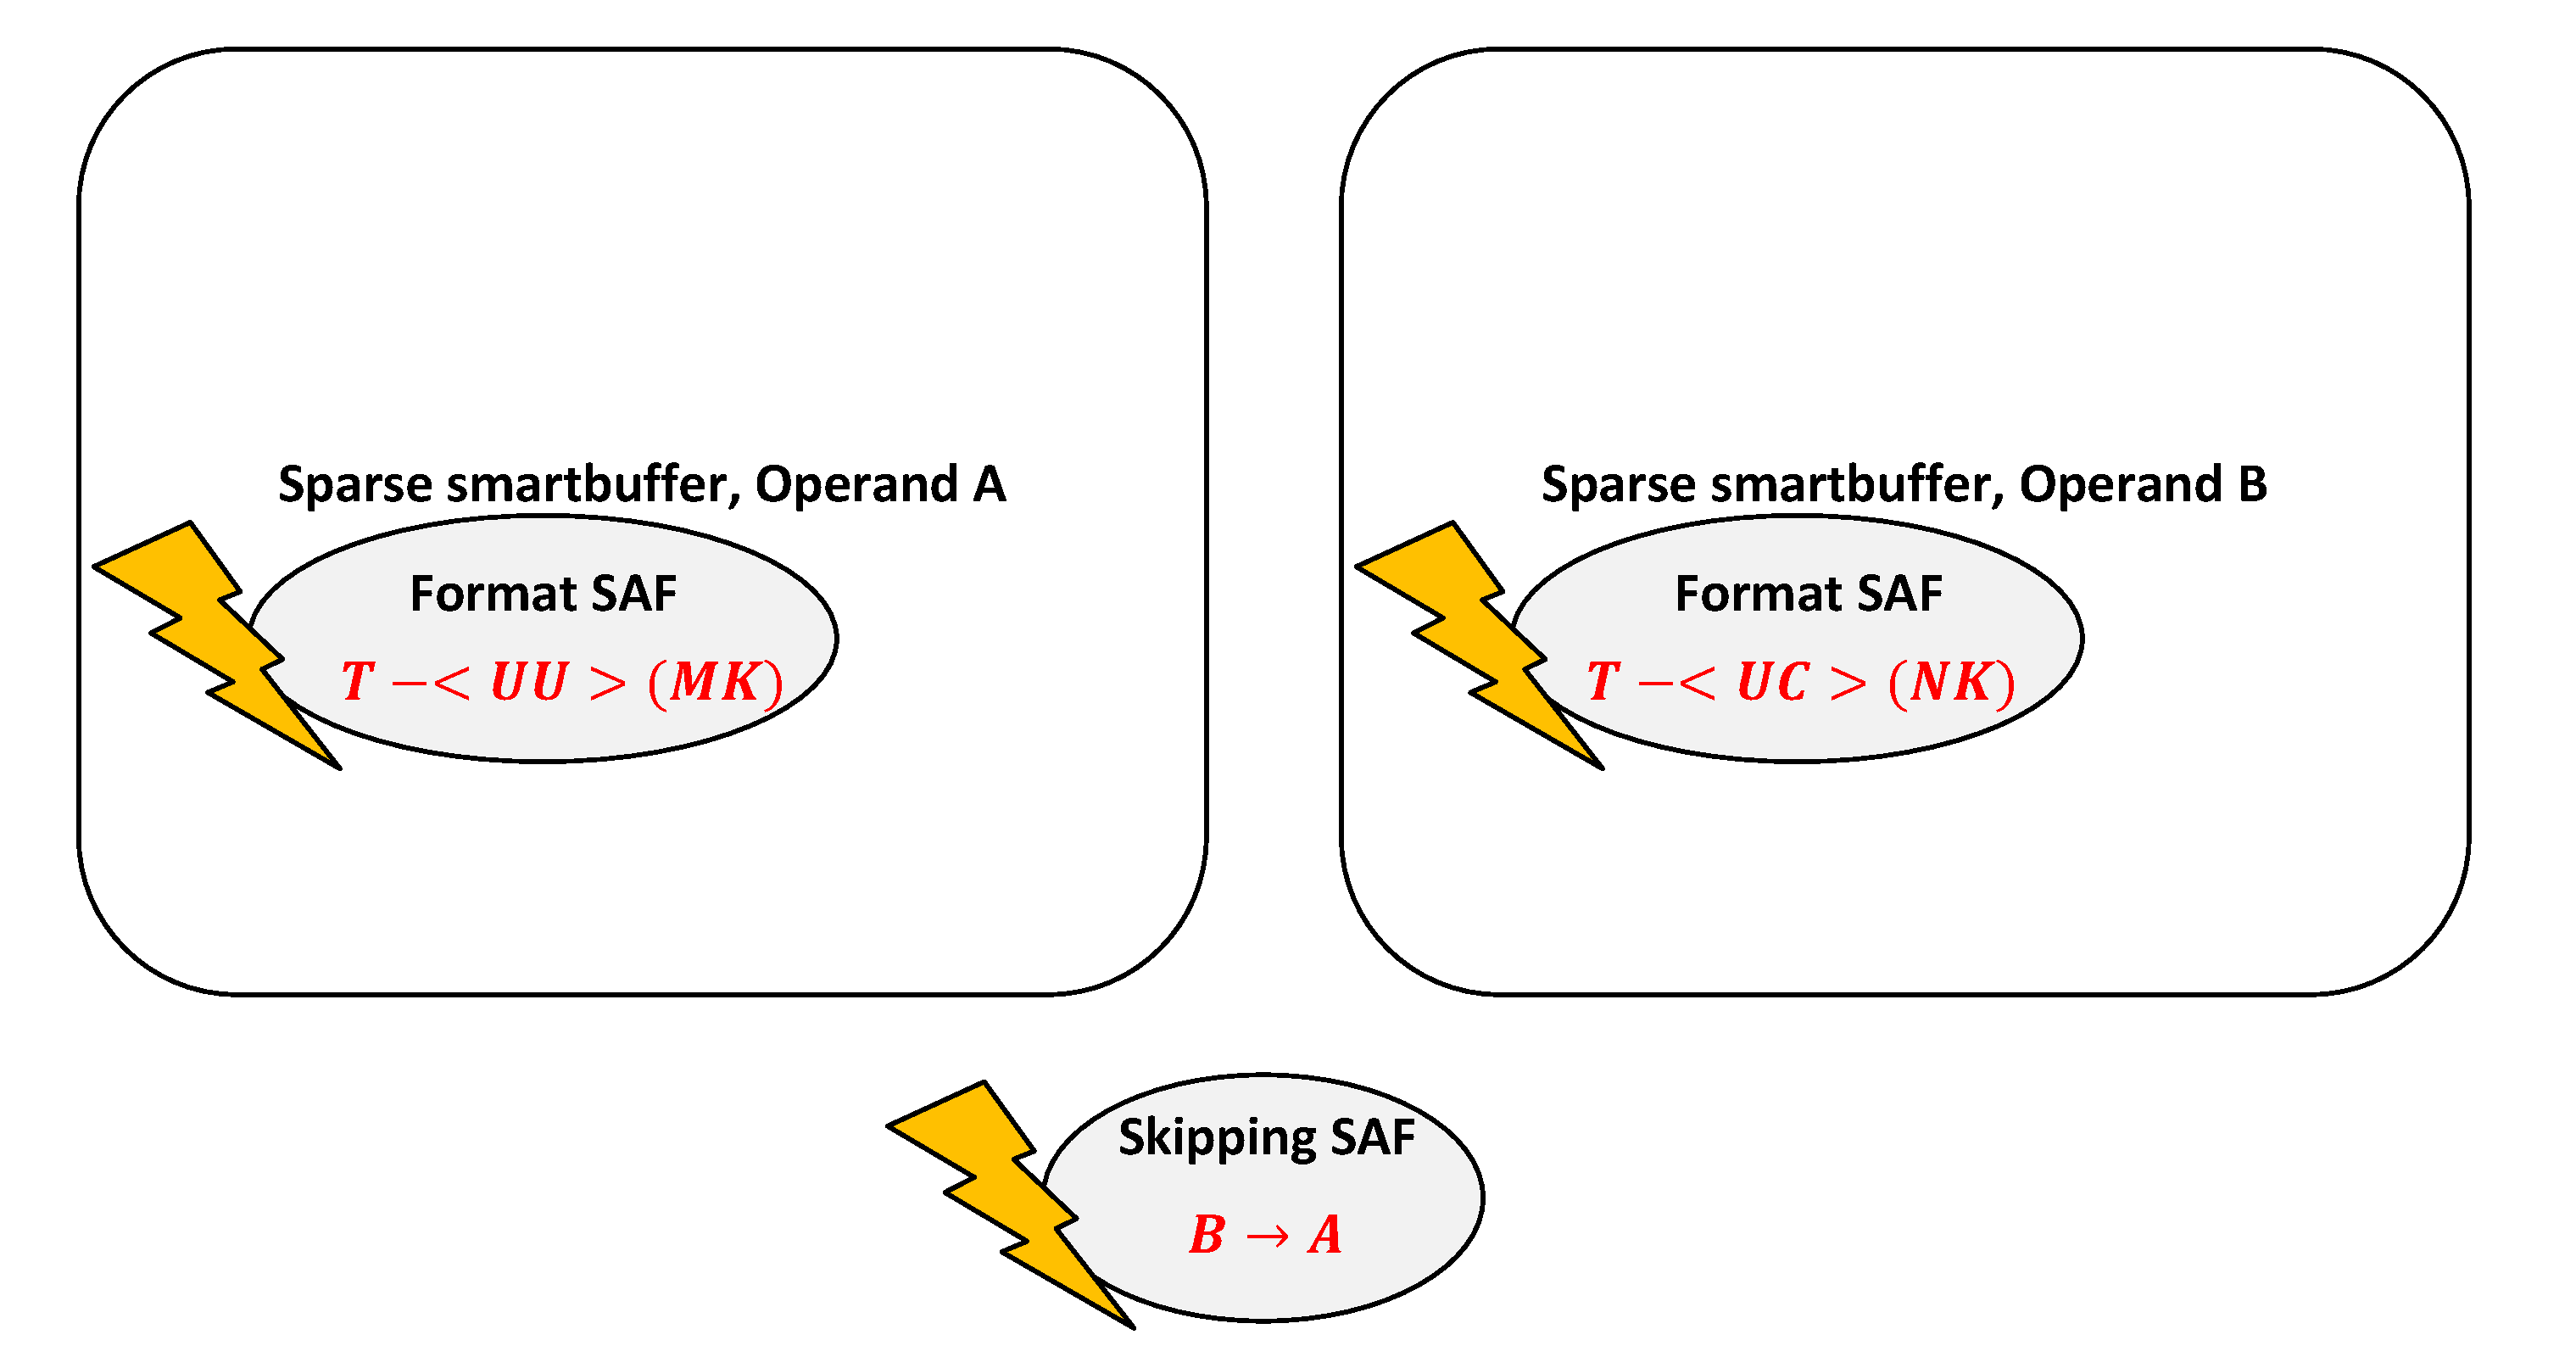
\includegraphics[width=\textwidth]{figures/safinfer_build_00saf.pdf}
\caption{\textbf{Sparseloop-style declarative specification of architecture and SAF optimizations.}}
\label{fig:safinfer_build_00saf}
\centering
\end{figure}

\clearpage

\begin{figure}[ht]
\includegraphics[width=\textwidth]{figures/safinference_build_01concretization.png}
\caption{\textbf{Concretization rule: replace declarative specs with high-level SAF microarchitecture blocks (FMT,SKIP.)}}
\label{fig:safinference_build_01concretization}
\centering
\end{figure}

\begin{figure}[ht]
\includegraphics[width=\textwidth]{figures/safinference_build_02fmtporttype.png}
\caption{\textbf{Port format(s) from attribute(s) rule: infer FMT block port formats from \textit{fmt\_list} attribute. }}
\label{fig:safinference_build_02fmtporttype}
\centering
\end{figure}



\begin{figure}[ht]
\includegraphics[width=\textwidth]{figures/safinference_build_03fmttopology.png}
\caption{\textbf{Topology inference from customization rule: infer FMT block implementation topology based on customization. }}
\label{fig:safinference_build_03fmttopology}
\centering
\end{figure}



\begin{figure}[ht]
\includegraphics[width=\textwidth]{figures/safinference_build_04mdparserportfmt.png}
\caption{\textbf{Wire-transitive rule: infer mdparsers' port formats from FMT block ports' formats.}}
\label{fig:safinference_build_04mdparserportfmt}
\centering
\end{figure}



\begin{figure}[ht]
\includegraphics[width=\textwidth]{figures/safinference_build_05mdparserfmtattr.png}
\caption{\textbf{Attribute from port format rule: infer mdparsers \textit{format} attributes' values from mdparsers ports' formats.}}
\label{fig:safinference_build_05mdparserfmtattr}
\centering
\end{figure}



\begin{figure}[ht]
\includegraphics[width=\textwidth]{figures/safinference_build_06mdparserstratcust.png}
\caption{\textbf{User customization rule: mdparsers' \textit{strategy} attributes are user-configurable free parameters.  }}
\label{fig:safinference_build_06mdparserstratcust}
\centering
\end{figure}



\begin{figure}[ht]
\includegraphics[width=\textwidth]{figures/safinference_build_07buffportfmt.png}
\caption{\textbf{Wire-transitive rule: infer architectural buffer-stub ports' formats from FMT block ports' formats. }}
\label{fig:safinference_build_07buffportfmt}
\centering
\end{figure}



\begin{figure}[ht]
\includegraphics[width=\textwidth]{figures/safinference_build_08skipportfmt.png}
\caption{\textbf{Wire-transitive rule: infer SKIP block ports' formats from architectural buffer stub ports' formats.}}
\label{fig:safinference_build_08skipportfmt}
\centering
\end{figure}



\begin{figure}[ht]
\includegraphics[width=\textwidth]{figures/safinference_build_09skipfmtattrs.png}
\caption{\textbf{Attribute from port format rule: infer SKIP block format attributes' values from SKIP blocks ports' formats.}}
\label{fig:safinference_build_09skipfmtattrs}
\centering
\end{figure}



\begin{figure}[ht]
\includegraphics[width=\textwidth]{figures/safinference_build_10skipoptfillscust.png}
\caption{\textbf{User customization rule: SKIP block's \textit{optimize\_fills} attribute is a user-configurable free parameter. }}
\label{fig:safinference_build_10skipoptfillscust}
\centering
\end{figure}



\begin{figure}[ht]
\includegraphics[width=\textwidth]{figures/safinference_build_11skiptopology.png}
\caption{\textbf{ Topology inference from customization rule: infer SKIP block implementation topology based on customization.}}
\label{fig:safinference_build_11skiptopology}
\centering
\end{figure}

\begin{figure}[ht]
\includegraphics[width=\textwidth]{figures/safinference_build_12isectlfpgenoneopt.png}
\caption{\textbf{Process-of-elimination rule: isectlf and both pgen1 units have only one supported customization; fill in unknown attributes. }}
\label{fig:safinference_build_12isectlfpgenoneopt}
\centering
\end{figure}

\begin{figure}[ht]
\includegraphics[width=\textwidth]{figures/safinference_build_13foptstratcust.png}
\caption{\textbf{User customization rule: fopt's \textit{strategy} attribute is a user-configurable free parameter. SAF microarchitecture taxonomic inference is complete.}}
\label{fig:safinference_build_13foptstratcust}
\centering
\end{figure}